%% Template for a preprint Letter or Article for submission
%% to the journal Nature.
%% Written by Peter Czoschke, 26 February 2004
%%

\documentclass{nature}
%\usepackage{subcaption}

%% make sure you have the nature.cls and naturemag.bst files where
%% LaTeX can find them

\bibliographystyle{naturemag}

\title{Death and taxa: time invariant differences in mammal species duration}

%% Notice placement of commas and superscripts and use of &
%% in the author list

\author{Peter D Smits$^{1}$}


\begin{document}

\maketitle

\begin{affiliations}
\item Committee on Evolutionary Biology, University of Chicago, Chicago, IL, USA.
\end{affiliations}

\begin{abstract}
%For Nature, the abstract is really an introductory paragraph set
%in bold type.  This paragraph must be ``fully referenced'' and
%less than 180 words for Letters.  This is the thing that is
%supposed to be aimed at people from other disciplines and is
%arguably the most important part to getting your paper past the
%editors.  End this paragraph with a sentence like ``Here we
%show...'' or something similar.
\end{abstract}

%Then the body of the main text appears after the intro paragraph.
%Figure environments can be left in place in the document.
%\verb|\includegraphics| commands are ignored since Nature wants
%the figures sent as separate files and the captions are
%automatically moved to the end of the document (they are printed
%out with the \verb|\end{document}| command. However, tables must
%be manually moved to the end of the document, after the addendum.

Why species go extinct at different rates remains one of the most fundamental questions in paleobiology \cite{Simpson1944,VanValen1973,Raup1991b,Raup1994,Quental2013,Wagner2014b}. Determining which and how biological traits influence extinction risk is vital for understanding the differential diversification of life during the Phanerozoic and for making predictions about species' vulnerability to anthropogenic impacts. 

Here I test if extinction is non-random with respect to organismal- and species-level traits during times of background extinction, if and which traits have time-invariant effects on species duration, and if extinction is taxon-age independent among Cenozoic mammals? I use a Bayesian hierarchical survival modeling approach to estimate the effects of organismal and species traits, time of origination, and shared evolutionary history on species duration while allowing for potentially age--dependent extinction. This is a statistical unification of both the dynamic and cohort survival approaches from paleontology \cite{VanValen1973,Raup1978}. Cenozoic mammals represent an ideal group and time period because their fossil record is well sampled, well resolved both temporally and spatially, and the ecology and taxonomy of individual species are generally understood \cite{Alroy2009,Alroy2000g,Liow2008,Smith2004,Quental2013,Alroy1998,Simpson1944,Tomiya2013,Marcot2014}. 

This study focuses on identifying the time-invariant effects of organismal and species traits on the expected duration of a species. A time-invariant effect is that when comparing taxa over a long time period there is a consistent effect that is generalizable over the entire period of interest. While the strength of that effect may vary over time, the direction does not change. For example, geographic range size has been identified as a generally time-invariant factor throughout the Phanerozoic, where large geographic range is associated with a decreased expected extinction risk \cite{Payne2007}. While it is almost certain that selection pressures vary with time, consistent effects reveal fundamental differences in fitness. Also, a shift in time-invariant factors may be an indicator of a change in ``macroevolutionary regime'' \cite{Jablonski1986} or a ``tipping point'' \cite{Barnosky2012a,Barnosky2011}, where the pattern of selection or ``rules'' are fundamentally changed or different between two time periods.

Periods of background extinction provide a great opportunity to study how traits are related to survival because they represent the majority of geologic time, remain relatively predictable, and change slowly \cite{Jablonski1986,Raup1988}. The Law of Constant Extinction \cite{VanValen1973} states that a taxon's extinction risk within a given adaptive zone is age-independent (memoryless). This law is the foundation for the Red Queen hypothesis as well as most approaches for quantifying extinction. However there is some evidence contrary to this law \cite{Finnegan2008}. By analyzing survival patterns within adaptive zones during periods of background extinction, it should be possible to both estimate the effects of various ecological strategies on survival and determine if extinction is age-independent or dependent. 

The organismal and species traits studied here are both dietary and locomotor categories, bioprovince occupancy, and body mass. Each of these traits describe different aspects of a species' adaptive zone such as energetic cost, population density, expected home range size, set of potential prey items, and dispersal ability \cite{Smith2004,Jernvall2004,Lyons2010}. It is expected that species with larger geographic ranges have lower extinction rates than species with smaller geographic ranges \cite{Jablonski1986,Harnik2013,Roy2009c}. However, organismal traits directly related to species--environment interactions may play an important role in determining extinction risk. By modeling extinction via traits related to environmental preference, the relative importance of species- and organismal-level properties can be elucidated. 

The Bayesian modeling framework used here allows for comparison of the marginal posterior estimates of each of the parameters acts as tests of the multiple trait effect hypotheses. All of these traits are analyzed with respect to the individual species origination cohort and phylogenetic position. From there the relative contribution species, cohort, and phylogeny to the unexplained variance can be estimated. Finally, the effect of time on extinction risk is explicitly modeled allowing for inference about the applicability of the Law of Constant Extinction \cite{VanValen1973}.

I found that dietary category has a large amount of variation in the pairwise differences of effects on expected duration (Fig. \ref{subfig:loco}). Carnivory appears to be associated with a greater expected duration than herbivory or insectivory, while approximately equal to or less than the expected duration of an omnivore. Omnivory is associated with greater expected duration than either herbivory or insectivory. Finally, herbivory and insectivory are associated with approximately equal effects on expected duration. 
These results sit nicely beside previous ones \cite{Price2012}. Given that carnivores and omnivores have approximately equal extinction risk, and it has been found previously that carnivores have a greater diversification rate than omnivores, this implies that carnivores have a greater origination rate than omnivores. This comparison implies that herbivores which have the greatest extinction risk must also have a very high origination rate in order to have the greatest diversification rate of these three categories. 

For locomotor category, arboreality appears to be associated with a lower expected duration than either scansoriality or a ground dwelling life habit (Fig. \ref{subfig:diet}). Scansoriality and a ground dwelling life habit have approximately equal expected durations. The effects of both body size and bioprovince occupancy on expected duration are best interpreted from estimates from the model fit standardized data (Fig. \ref{fig:eff_other}). As expected, bioprovince occupancy has the largest effect on expected species duration/extinction risk. The other factors all appear to have small effect sizes which is also consistent with expectations. Body size has a very small, near zero effect on expected duration, similar to the lack of relationship between body size and generic duration \cite{Tomiya2013}. These results consistent with the hypotheses that arboreality is associated with a greater expected extinction risk than either with scansoriality and ground dwelling taxa. Importantly, scansoriality appears to not influence any difference in extinction risk when compared with ground dwelling taxa. This can be interpreted that arboreal taxa, which require a specific kind of environment, may be more prone to extinction because the lack of permanency of those environments may prevent species persistence. 

The large difference in time-invariant extinction risk between omnivores and both herbivores and insectivores is most likely related to the concept of ``survival of the unspecialized'' where less specialized taxa have lower extinction risks \cite{Liow2004a,Simpson1944}. Because larger effects are easier to identify in coarse or small data sets, the magnitude of this effect also explains both the early identification and origin of this hypothesis of time-invariant effects on survival \cite{Simpson1944}. The very weak if non-existent effect of body size on extinction risk, which can be considered not ``significant'', is consistent with some previous results \cite{Tomiya2013}. The direction/sign of the modal estimate of effect is not consistent with the prediction of increase in extinction risk associated with increase in body size \cite{Liow2008}. Importantly, however, the other studies were performed at the generic-level which may or may not involve different processes that are not included in this species-level model.

Of the three sources of variance present in the model, variation in individual species accounts for approximately 70\% of observed variance (Fig. \ref{fig:vpc}). Both cohort and phylogenetic effects account for the other 30\% of the observed variance. Both of these factors are related to some aspect of the relationship between taxa, either temporal and through shared evolutionary history. While both of these effects are the source of approximately 15\% of observed variance individually, the total combined effect of these factors indicates that neither can be ignored. As \(VPC_{phylo}\) is equivalent to phylogenetic heritability and is greater than 0, it is not appropriate to ignore phylogeny when modeling survival in paleontological studies \cite{Housworth2004} even though this is commonly done \cite{Alroy2009,Foote2013,Jablonski2006a,Hunt2007a,Liow2008,Payne2007}. An addition 10-15\% of unexplained variance was due to shared origination cohort. Between these two sources of variance, it is clear that a shared evolutionary history and temporal occurrence are non-ignorable in paleontological studies or survival. Modeling phylogeny as a hierarchical effect, as done here, is a very simple and interpretable means of integrating phylogenetic information into any and all regression models \cite{Lynch1991,Housworth2004} and is most likely ideal for most paleontological studies.

Because the estimate of the Weibull shape parameter, \(\alpha\), is greater than 1 extinction risk is expected to increase with taxon age (Table \ref{tab:post_sum}). The estimate of \(\alpha\) is also rather tightly constrained, having a small posterior standard deviation. \(\alpha\) is related to the strength of time on extinction risk and is a key parameter in the hazard function \(h(t)\) which can be interpreted as the rate, or approximate probability, of an individual of age \(t\) going extinct. As the value of \(\alpha\) is between 1 and 1.5, extinction risk for a given species only gradually increases with age (Fig. \ref{fig:haz}). This result has two possible explanations: (1) older taxa being aged out or out competed by younger taxa, or (2) as an artifact of the minimum resolution of the fossil record.

The hypothesis that older taxa are being outcompeted or replaced by younger taxa is also consistent with the some recent results \cite{Wagner2014b,Quental2013}, both of which require that older taxa have a greater extinction risk than younger taxa.

The other possible explanation for the inferred increase in extinction risk with species age is the minimum resolution which might cause an upward bias in estimates of the Weibull shape parameter \(\alpha\) \cite{Sepkoski1975}, an effect which can be observed by the initial plateau in the K-M estimate of \(S(t)\) for the observed (Fig. \ref{fig:ppc_surv}). This plateau is a hallmark of the original paleontological survival analyses \cite{VanValen1973} which was identified as partially a product of minimum resolution of the fossil records of the different studied groups.

Given this known biasing factor and previous results \cite{Wagner2014b,Quental2013}, I hypothesize that the inferred pattern is most likely a combination of these two explanations working on concert. In order to determine the relative importance of these two explanations, more work is required into approaches for directly modeling the minimum resolution of the fossil record.

The estimates for the individual cohort effects show a weak pattern of increased extinction risk in older Cenozoic cohorts and decreased extinction risk in younger cohorts (Fig. \ref{fig:eff_cohort}). However, this pattern is not very strong as there is a large amount of variation, particularity for older cohorts. For example, note the two cohorts between 50 and 55 My that have a much lower extinction risk than other cohorts of similar age. However, it is interesting to note that the apparent shift from older cohorts with a higher extinction risk to younger cohorts with lower extinction risk is approximately 30 Mya or the Paleogene--Neogene boundary. This transition is marked by the opening up of the landscape and the rise of grazers and the decline heavily forested environments. This shift may underly the inferred increased extinction risk associated with arboreal species compared to ground dwelling or scansorial species (Fig. \ref{subfig:loco}). However, because the model used here does not allow for change in time-invariant effects, I cannot identify this transition as a tipping point or shift in selective regime \cite{Barnosky2012a,Barnosky2011}.

One of the open questions in paleobiology and macroecology is whether the current biodiversity crisis qualified as a mass extinction \cite{Alroy2010,Barnosky2011,Barnosky2012a}. Because change in the magnitude of extinction risk is not necessarily the best indicator of a shift from background to mass extinction \cite{Wang2003}, it is more fruitful to look for changes in the direction selection, loss of a selective pressure, or appearance of novel selective pressures. Comparison of the estimated effects of organismal- and species-level traits analyzed here with previous studies demonstrates a mixture of congruence and incongruence. 

As expected, large range size is always associated with lower extinction risk in the Recent \cite{Fritz2009,Fritz2010b,Liow2009,Purvis2000a}. While I found that body size has no time-invariant effect on extinction risk, large body size is associated with increased extinction risk in the Recent, though this is variable across environments and clades \cite{Liow2009,Fritz2009,Purvis2000a}. A higher trophic level (e.g. carnivory versus herbivory) is associated with greater extinction risk in Primates and Carnivora \cite{Purvis2000a} which is not congruous with the results found here that carnivores have lower extinction risk than herbivores. Finally, phylogeny has been found to be a factor underlying current mammal species extinction risk, though this effect seems much greater in the Recent than for the whole Cenozoic \cite{Fritz2010b}. Note that the phylogeny of Recent mammals is much better than the primarily taxonomy based phylogeny used here, which may partially account for the difference in effect.

How many of these incongruities are within the standard range of time-variant effects is unknown, though these comparisons across multiple factors do point to our arrival at a tipping point \cite{Barnosky2012a,Barnosky2011} and potentially a shift in macroevolutionary regime \cite{Jablonski1986}.


There are a few data quality concerns in this study which are also inherent to almost any paleontological study. Almost all of the body mass estimates were obtained using published regression equations that estimate mass from some other body part (e.g. tooth). These estimates are known with error, which was not included in the model. If the standard deviation of the residuals from each of these regression equations was known, it would be possible to directly model this as measurement error \cite{Gelman2013d} though this greatly adds to model complexity and decreases some amount of interpretability.  Also phylogeny used here is only a coarse, baseline estimate of the actual species relationships. Because of this, the analysis of phylogenetic effect on survival represents a minimum eistimate. As it stands though, these results point to the importance of including shared evolutionary history in diversification models.


There are many processes encompassed by background extinction and identifying the exact cause of any one species' reason for extinction is extremely difficult. By focusing on estimating the effects of different ecologies and historical factors on average extinction risk, it is possible to better understand what processes may have driven the resulting pattern of selection (i.e. diversity). Here, I focused on time-invariant factors and their relation to biological selectivity of extinction, possible reasons for the observed time-invariant effects, and the effects of taxon-age on extinction risk. I found that some organismal- and species-level traits such as omnivory and large geographic range size have time-invariant effects on mammal species extinction risk. I also found that there are small but non-ignorable effects of cohort and phylogeny. Finally, I found putative evidence of increasing extinction risk with species age, though this result may be partially due to the minimum resolution of the fossil record itself \cite{Sepkoski1975}.


%\begin{figure}
%\caption{Each figure legend should begin with a brief title for
%the whole figure and continue with a short description of each
%panel and the symbols used. For contributions with methods
%sections, legends should not contain any details of methods, or
%exceed 100 words (fewer than 500 words in total for the whole
%paper). In contributions without methods sections, legends should
%be fewer than 300 words (800 words or fewer in total for the whole
%paper).}
%\end{figure}
%
%\section*{Another Section}
%
%Sections can only be used in Articles.  Contributions should be
%organized in the sequence: title, text, methods, references,
%Supplementary Information line (if any), acknowledgements,
%interest declaration, corresponding author line, tables, figure
%legends.
%
%Spelling must be British English (Oxford English Dictionary)
%
%In addition, a cover letter needs to be written with the
%following:
%\begin{enumerate}
% \item A 100 word or less summary indicating on scientific grounds
%why the paper should be considered for a wide-ranging journal like
%\textsl{Nature} instead of a more narrowly focussed journal.
% \item A 100 word or less summary aimed at a non-scientific audience,
%written at the level of a national newspaper.  It may be used for
%\textsl{Nature}'s press release or other general publicity.
% \item The cover letter should state clearly what is included as the
%submission, including number of figures, supporting manuscripts
%and any Supplementary Information (specifying number of items and
%format).
% \item The cover letter should also state the number of
%words of text in the paper; the number of figures and parts of
%figures (for example, 4 figures, comprising 16 separate panels in
%total); a rough estimate of the desired final size of figures in
%terms of number of pages; and a full current postal address,
%telephone and fax numbers, and current e-mail address.
%\end{enumerate}
%
%See \textsl{Nature}'s website
%(\texttt{http://www.nature.com/nature/submit/gta/index.html}) for
%complete submission guidelines.
%
\begin{methods}

  \subsection{Data and covariate information.}
  Fossil occurrence information was downloaded from the Paleobiology Database (PBDB). This data set was filtered so that only occurrences identified to the species-level, excluding all ``sp.''-s. All aquatic and volant taxa were also excluded. Additionally, all occurrences without latitude and longitude information were excluded.

  Species dietary and locomotor category assignments were based on assignments in initial the PBDB which were then reassigned into coarser categories.

  All individual fossil occurrences were assigned to 2 My bins ranging through the entire Cenozoic. Species duration was measured as the number of bins from the first occurrence to the last occurrence, inclusive. This bin size was chosen because it approximately reflects the resolution of the North American Cenozoic mammal fossil record \cite{Alroy2009,Marcot2014}. The youngest cohort, 0-2 My, was excluded from analysis.

  Species body size estimates were sourced from a large selection of primary literature and data base compilations, principally the PBDB, the Neogene Old World Mammal database, and other large scale data collection efforts \cite{Jones2009c,Smith2004c,Raia2012f,Freudenthal2013,McKenna2011}. 

  For each 2 My bin, a bipartite biogeographic network was created between species occurrences and spatial units, defined as 2x2 latitude--longitude grid cells from an azimuthal equal-area map projection. Emergent bioprovinces within the biogeographic occurrence network were identified using the map equation \cite{Rosvall2008,Vilhena2013}. A bioprovince is a set of species--locality connections that are more interconnected within the group than without.

  As there is no single, combined formal phylogenetic hypothesis of all Cenozoic fossils mammals from North America, it was necessary to construct a semi-formal supertree. This was done by combining taxonomic information for all the observed species and a few published, species level phylogenies \cite{Raia2012f,Janis1998,Janis2008}.

%Put methods in here.  If you are going to subsection it, use
%\verb|\subsection| commands.  Methods section should be less than
%800 words and if it is less than 200 words, it can be incorporated
%into the main text.

  \subsection{Survival model.}

  Species durations were modeled as being drawn from a Weibull distribution with two parameters: shape \(\alpha\) and scale \(\sigma\). \(\sigma\) was parameterized as a regression model with an exponential link function because it is defined only for values greater than 0. This regression model included eight species-level coefficients for the covariates (dietary and locomotor categories, body size, mean bioprovince occupancy) along with an intercept term. Both continuous covariates were standardized by subtracting the mean value and dividing by 2 times the standard deviation so that the inferred values were comparable with the coefficients from the binary variables \cite{Gelman2007}. Each of these coefficients was given a weakly informative normally distributed prior.
  
  Additionally, a hierarchical term was included for origination cohort along with an individual effect for phylogeny. Cohorts were consider drawn from a shared normal distribution with mean 0 and standard deviation estimated from the data. This standard deviation term was given a weakly informative half-Cauchy prior \cite{Gelman2013d}. Individual phylogenetic effect was considered drawn from a multivariate normal distribution with mean vector of all 0's and covariance matrix being the phylogenetic covariance matrix multiplied by an unknown constant \cite{Lynch1991,Housworth2004}.

  Species that are still extant were right censored while species that occupied only one 2 My bin were left censored to reflect the minimum resolution of the fossil record.

  Parameters were estimated using a variant Markov-chain Monte Carlo routine implemented in the Stan programming language \cite{2014stan}. Model adequacy was assessed through a multiple posterior predictive checks to determine if the model accurately reflected the observed species durations \cite{Gelman2013d}. 

  %Variance partitioning was done using a variant of a known randomization approach \cite{Goldstein2002}.


%Here is a description of a specific method used.  Note that the
%subsection heading ends with a full stop (period) and that the
%command is \verb|\subsection{}| not \verb|\subsection*{}|.

\end{methods}


\bibliography{biblio,packages}


%% Here is the endmatter stuff: Supplementary Info, etc.
%% Use \item's to separate, default label is "Acknowledgements"

\begin{addendum}
\item P.D.S would like to thank M. Foote, K. Angielczyk, R. Ree, P.D. Polly for discussion. J. Alroy and Fossilworks/the Paleobiology Database for data gathering, entry, and availability.
\item[Competing Interests] The authors declare that they have no
  competing financial interests.
\item[Correspondence] Correspondence and requests for materials
  should be addressed to P.D.S.~(email: psmits@uchicago.edu).
\end{addendum}

%%
%% TABLES
%%
%% If there are any tables, put them here.
%%

% latex table generated in R 3.1.2 by xtable 1.7-4 package
% Thu Jan  8 17:45:30 2015
\documentclass{article}
\begin{document}
\begin{table}[c]
  \centering
  \begin{tabular}{ l l r r r r r r r r }
    parameter & effect & mean & sd & 2.5\% & 25\% & 50\% & 75\% & 97.5\% & \(\hat{R}\) \\ 
    \hline
    \(\alpha\) & ``age'' &1.29 & 0.03 & 1.23 & 1.27 & 1.29 & 1.31 & 1.36 & 1.02 \\ 
    \hline
    \(\beta_{0}\) & arboreal/carnivore & -0.78 & 0.14 & -1.06 & -0.88 & -0.78 & -0.69 & -0.50 & 1.01 \\ 
    \(\beta_{o}\) & occupancy & -0.57 & 0.08 & -0.73 & -0.63 & -0.57 & -0.52 & -0.41 & 1.00 \\ 
    \(\beta_{size}\) & body size & 0.01 & 0.05 & -0.08 & -0.02 & 0.02 & 0.05 & 0.11 & 1.00 \\ 
    \(\beta_{g}\) & ground dwelling & -0.27 & 0.09 & -0.45 & -0.33 & -0.27 & -0.21 & -0.08 & 1.00 \\ 
    \(\beta_{s}\) & scansorial & -0.21 & 0.11 & -0.43 & -0.28 & -0.21 & -0.14 & -0.01 & 1.00 \\ 
    \(\beta_{h}\) & herbivore & 0.08 & 0.09 & -0.09 & 0.02 & 0.08 & 0.14 & 0.26 & 1.00 \\ 
    \(\beta_{i}\) & insectivore & 0.08 & 0.11 & -0.13 & 0.01 & 0.08 & 0.15 & 0.29 & 1.00 \\ 
    \(\beta_{o}\) & omnivore & -0.13 & 0.10 & -0.34 & -0.20 & -0.13 & -0.06 & 0.07 & 1.00 \\ 
    \hline
    \(\sigma_{c}\) & sd cohort & 0.34 & 0.07 & 0.24 & 0.30 & 0.33 & 0.38 & 0.50 & 1.00 \\ 
    \(\sigma_{p}\) & sd phylogeny & 0.11 & 0.06 & 0.02 & 0.07 & 0.10 & 0.15 & 0.25 & 1.07 \\ 
    \hline
  \end{tabular}
\end{table}
\end{document}


\begin{figure}[ht]
  %\centering
  %\includegraphics[height = 0.5\textheight, width = \textwidth, keepaspectratio = true]{figure/residual_plot}
  \caption{Deviance residuals from the fitted survival model. Each graph depicts the residuals from single draws from the posteriors distributions of all estimated parameters. Positive values indicate an under estimate of the observed duration, while negative values indicate an over estimate of the observed duration. Twelve difference examples are provided here to indicate the lack of individual observation based biases.}
  \label{fig:ppc_res}
\end{figure}

\begin{figure}[ht]
  %\centering
  %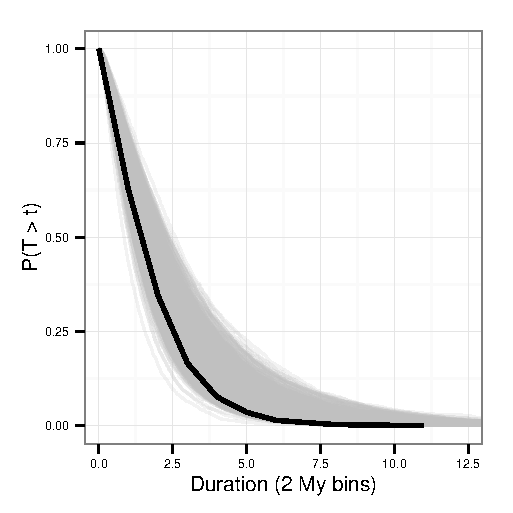
\includegraphics[height = 0.5\textheight, width = \textwidth, keepaspectratio = true]{figure/survival_function}
  \caption{Comparison between K-M estimate of survival function (black) from the observed versus K-M estimates from 100 simulated data sets using the fitted model (dark grey). Simulated data sets were generated by drawing parameter values randomly from their estimated posteriors and using the observed covariate information to estimate durations for all the observed species. On the left are the results from the full survival model, while on the right are the results from a simplified model where duration follows an exponential distribution and there is no phylogenetic effect.}
  \label{fig:ppc_surv}
\end{figure}

\begin{figure}[ht]
  %\centering
  %\includegraphics[height = 0.5\textheight, width = \textwidth, keepaspectratio = true]{figure/quant_ppc}
  \caption{The results of additional posterior predictive checks for four summaries of the observed durations, as labeled. Blue vertical indicate the observed value. None of the observed are significantly different from the posterior predictive distributions.}
  \label{fig:ppc_quant}
\end{figure}

\begin{figure}[ht]
  %\centering
  %\begin{subfigure}[b]{0.4\textwidth}
  %  \caption{}
  %  \includegraphics[height = 0.5\textheight, width = \textwidth, keepaspectratio = true]{figure/loco_diff_est}
    \label{subfig:loco}
  %\end{subfigure}
  %\begin{subfigure}[b]{0.4\textwidth}
  %  \caption{}
  %  \includegraphics[height = 0.5\textheight, width = \textwidth, keepaspectratio = true]{figure/diet_diff_est}
    \label{subfig:diet}
  %\end{subfigure}
  \caption{Pairwise differences in effect of the locomotor (\ref{subfig:loco}) and dietary categories (\ref{subfig:diet}) on expected duration from 1000 samples from the posterior distribution. Comparisons of locomotor categories, from top to bottom (\ref{subfig:loco}), are: arboreal versus ground dwelling, arboreal versus scansorial, and ground dwelling versus scansorial. For dietary category, from top to bottom (\ref{subfig:diet}): carnivore versus herbivore, carnivore versus insectivore, carnivore versus omnivore, herbivore versus insectivore, herbivore versus omnivore, and insectivore versus omnivore. Values to the left indicate that the first category is expected to have a greater duration than the second, while values to the right indicate that the first category is expected to have a shorter duration.}
  \label{fig:trait_est}
\end{figure}

\begin{figure}[ht]
  %\centering
  %\includegraphics[height = 0.5\textheight, width = \textwidth, keepaspectratio = true]{figure/other_est}
  \caption{}
  \label{fig:eff_other}
\end{figure}

\begin{figure}[ht]
  %\centering
  %\includegraphics[height = 0.5\textheight, width = \textwidth, keepaspectratio = true]{figure/cohort_est}
  \caption{Summaries of estimated individual cohort effect posteriors. Depicted are medians and 80\% credible intervals of the estimated posterior distributions. High values correspond to shorter species durations while lower values correspond to greater species durations compared to the mean duration. Lines are placed at the middle of the 2 My origination cohorts.}
  \label{fig:eff_cohort}
\end{figure}

\begin{figure}[ht]
  %\centering
  %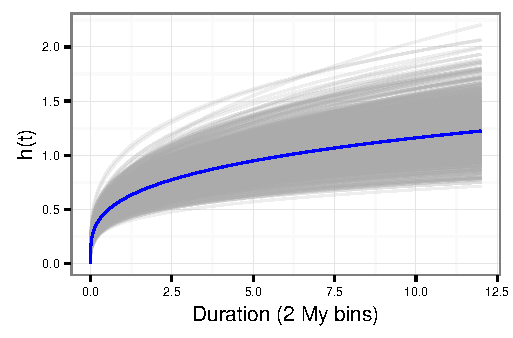
\includegraphics[height = 0.5\textheight, width = \textwidth, keepaspectratio = true]{figure/haz_est}
  \caption{100 estimates of the hazard function (\(h(t\)) for the observed species mean (grey), along with the median estimated hazard function. \(h(t)\) is an estimate of the rate at which a species of age \(t\) is expected to go extinct. Hazard functions were estimated from random draws from the estimated posterior distributions and evaluated with all covariate information set to 0, which corresponds to the expected duration of the mean species.}
  \label{fig:haz}
\end{figure}

\begin{figure}[ht]
  %\centering
  %\includegraphics[height = 0.5\textheight, width = \textwidth, keepaspectratio = true]{figure/variance_est}
  \caption{Estimates of the variance partitioning coefficients for the three different sources of variance: species, cohort, and phylogeny. Higher values correspond to greater contribution to total observed variance. Each of the estimates is a distribution of 1000 approximating simulations due to the model's non-normality.}
  \label{fig:vpc}
\end{figure}

\end{document}
